\noindent\resizebox{\textwidth}{!}{
  \begin{tikzpicture}
    \draw[use as bounding box, transparent] (-4.8,-1.8) rectangle (20.2, 3.2);

    % Define the macro.
    % 1st argument: Height and width of the layer rectangle slice.
    % 2nd argument: Depth of the layer slice
    % 3rd argument: X Offset --> use it to offset layers from previously drawn layers.
    % 4th argument: Options for filldraw.
    % 5th argument: Text to be placed below this layer.
    % 6th argument: Y Offset --> Use it when an output needs to be fed to multiple layers that are on the same X offset.

    \newcommand{\networkLayer}[6]{
      \def\a{#1} % Used to distinguish input resolution for current layer.
      \def\b{0.02}
      \def\c{#2} % Width of the cube to distinguish number of input channels for current layer.
      \def\t{#3} % X offset for current layer.
      \def\d{#4} % Y offset for current layer.

      % Draw the layer body.
      \draw[line width=0.3mm](\c+\t,0,\d) -- (\c+\t,\a,\d) -- (\t,\a,\d);                                                      % back plane
      \draw[line width=0.3mm](\t,0,\a+\d) -- (\c+\t,0,\a+\d) node[midway,below] {#6} -- (\c+\t,\a,\a+\d) -- (\t,\a,\a+\d) -- (\t,0,\a+\d); % front plane
      \draw[line width=0.3mm](\c+\t,0,\d) -- (\c+\t,0,\a+\d);
      \draw[line width=0.3mm](\c+\t,\a,\d) -- (\c+\t,\a,\a+\d);
      \draw[line width=0.3mm](\t,\a,\d) -- (\t,\a,\a+\d);

      % Recolor visible surfaces
      \filldraw[#5] (\t+\b,\b,\a+\d) -- (\c+\t-\b,\b,\a+\d) -- (\c+\t-\b,\a-\b,\a+\d) -- (\t+\b,\a-\b,\a+\d) -- (\t+\b,\b,\a+\d); % front plane
      \filldraw[#5] (\t+\b,\a,\a-\b+\d) -- (\c+\t-\b,\a,\a-\b+\d) -- (\c+\t-\b,\a,\b+\d) -- (\t+\b,\a,\b+\d);

      % Colored slice.
      \ifthenelse {\equal{#5} {}}
      {} % Do not draw colored slice if #4 is blank.
      {\filldraw[#5] (\c+\t,\b,\a-\b+\d) -- (\c+\t,\b,\b+\d) -- (\c+\t,\a-\b,\b+\d) -- (\c+\t,\a-\b,\a-\b+\d);} % Else, draw a colored slice.
    }

    \colorlet{inp}{red!70!white}
    \colorlet{conv}{blue!70!white}
    \colorlet{pool}{yellow}
    \colorlet{upsample}{orange}
    \colorlet{out}{green!70!white}

    % INPUT
    \node[] (input image) at (-3.75,0.5) {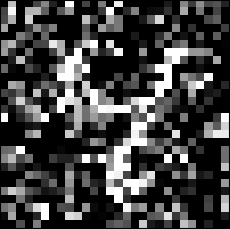
\includegraphics[height=30mm]{noisy_num.png}};
    \networkLayer{3.0}{0.03}{-0.5}{0.0}{color=inp}{}

    % ENCODER
    \networkLayer{3.0}{0.1}{0.0}{0.0}{color=conv}{}    % S1
    \networkLayer{3.0}{0.1}{0.2}{0.0}{color=pool}{}        % S2
    \networkLayer{2.5}{0.2}{0.6}{0.0}{color=conv}{}    % S1
    \networkLayer{2.5}{0.2}{0.9}{0.0}{color=pool}{}        % S2
    \networkLayer{2.0}{0.4}{1.3}{0.0}{color=conv}{}    % S1
    \networkLayer{2.0}{0.4}{1.8}{0.0}{color=pool}{}        % S2
    \networkLayer{1.5}{0.8}{2.3}{0.0}{color=conv}{}    % S1
    \networkLayer{1.5}{0.8}{3.2}{0.0}{color=pool}{}        % S2
    \networkLayer{1.0}{1.5}{4.1}{0.0}{color=conv}{}    % S1
    \networkLayer{1.0}{1.5}{5.7}{0.0}{color=pool}{}        % S2

    % DECODER
    \networkLayer{1.0}{1.5}{7.7} {0.0}{color=conv}{} % S1
    \networkLayer{1.0}{1.5}{9.3} {0.0}{color=upsample}{}       % S2
    \networkLayer{1.5}{0.8}{11.2}{0.0}{color=conv}{} % S1
    \networkLayer{1.5}{0.8}{12.1}{0.0}{color=upsample}{}       % S2
    \networkLayer{2.0}{0.4}{13.3}{0.0}{color=conv}{}       % S1
    \networkLayer{2.0}{0.4}{13.8}{0.0}{color=upsample}{}       % S2
    \networkLayer{2.5}{0.2}{14.8}{0.0}{color=conv}{}       % S1
    \networkLayer{2.5}{0.2}{15.1}{0.0}{color=upsample}{}       % S2
    \networkLayer{3.0}{0.1}{15.8}{0.0}{color=conv}{}       % S1
    \networkLayer{3.0}{0.1}{16}  {0.0}{color=upsample}{}       % S2

    % OUTPUT
    \networkLayer{3.0}{0.05}{17}{0.0}{color=out}{}          % Pixelwise segmentation with classes.
    \node[] (output image) at (19,0.5) {
\includegraphics[height=30mm]{clean_num.png}};

  \end{tikzpicture}
}
%%% Local Variables:
%%% mode: latex
%%% TeX-master: "../figs"
%%% End:
